\documentclass[tikz,border=2pt]{standalone}
% Preámbulo común de los diagramas TikZ (misma paleta y letra que las notas)
\usepackage[T1]{fontenc}\usepackage[utf8]{inputenc}
\usepackage{libertinus}\usepackage{libertinust1math}
\usepackage[defaultsans,scale=0.92]{lato}
\usepackage{amsmath,amssymb,bm}
\usepackage{tikz}\usetikzlibrary{calc,positioning,arrows.meta,shapes.geometric,decorations.pathreplacing,decorations.pathmorphing,fit,backgrounds}
\definecolor{snlazul}{HTML}{1E5AA8}\definecolor{snlnoche}{HTML}{14213D}\definecolor{snlvioleta}{HTML}{6C4AB6}
\definecolor{snlcoral}{HTML}{D1495B}\definecolor{snlambar}{HTML}{E09F3E}\definecolor{snlverde}{HTML}{2A9D8F}
\definecolor{snlteal}{HTML}{0F7173}\definecolor{snlgris}{HTML}{5C677D}\definecolor{snlfondo}{HTML}{F4F6FA}
\tikzset{>={Stealth[length=2.2mm]},
  bloque/.style={draw=#1,fill=#1!8,thick,rounded corners=2pt,minimum height=11mm,minimum width=20mm,align=center,font=\small},
  bloque/.default=snlazul,
  suma/.style={draw=snlnoche,thick,circle,inner sep=0pt,minimum size=5mm},
  flecha/.style={->,thick,draw=snlnoche},
  etq/.style={font=\small,text=snlnoche},
  nota/.style={font=\footnotesize\sffamily,text=snlgris,align=center}}

\begin{document}
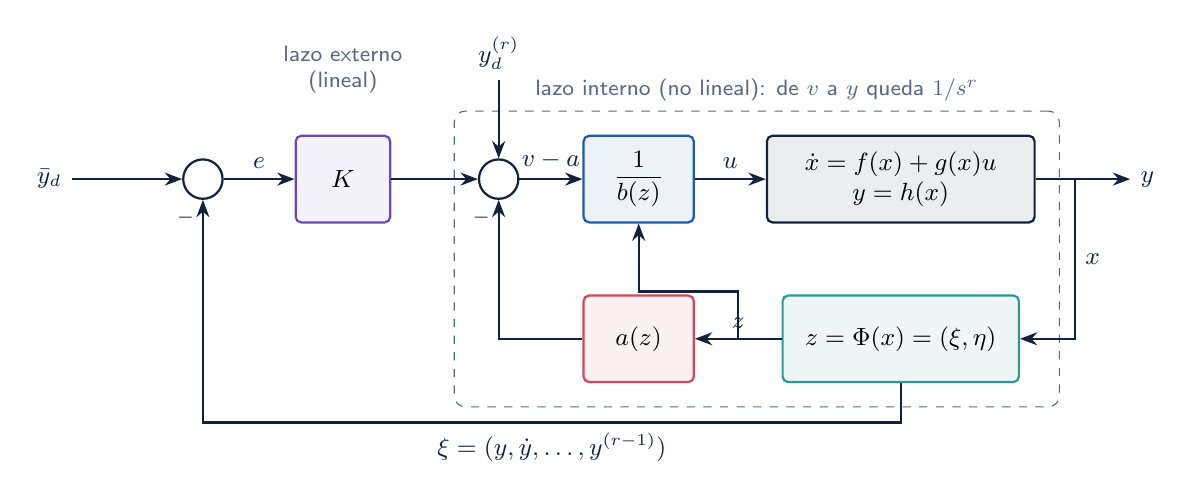
\begin{tikzpicture}
 \node[suma] (s1) {};
 \node[bloque=snlvioleta,right=9mm of s1,minimum width=12mm] (K) {$K$};
 \node[suma,right=11mm of K] (s2) {};
 \node[bloque=snlazul,right=8mm of s2,minimum width=14mm] (beta) {$\dfrac{1}{b(z)}$};
 \node[bloque=snlnoche,right=9mm of beta,minimum width=34mm] (P) {$\dot x=f(x)+g(x)u$\\$y=h(x)$};
 \node[bloque=snlcoral,below=9mm of beta,minimum width=14mm] (a) {$a(z)$};
 \node[bloque=snlverde,below=9mm of P,minimum width=30mm] (Phi) {$z=\Phi(x)=(\xi,\eta)$};
 \draw[flecha] ($(s1.west)+(-14mm,0)$) node[left,etq]{$\bar y_d$} -- (s1);
 \draw[flecha] (s1) -- node[above,etq]{$e$} (K);
 \draw[flecha] (K) -- node[above,etq]{} (s2);
 \draw[flecha] ($(s2.north)+(0,10mm)$) node[above,etq]{$y_d^{(r)}$} -- (s2);
 \draw[flecha] (s2) -- node[above,etq]{$v-a$} (beta);
 \draw[flecha] (beta) -- node[above,etq]{$u$} (P);
 \draw[flecha] (P.east) -- ++(12mm,0) node[right,etq]{$y$};
 \draw[flecha] ($(P.east)+(5mm,0)$) |- node[pos=0.25,right,etq]{$x$} (Phi.east);
 \draw[flecha] (Phi.south) -- ++(0,-5mm) -| node[pos=0.25,below,etq]{$\xi=(y,\dot y,\dots,y^{(r-1)})$} (s1.south);
 \draw[flecha] (Phi.west) -- node[above,etq]{$z$} (a.east);
 \draw[flecha] ($(Phi.west)!0.5!(a.east)$) -- ++(0,6mm) -| (beta.south);
 \draw[flecha] (a.west) -| (s2.south);
 \node[font=\scriptsize,text=snlnoche] at ($(s1.south)+(-2.2mm,-2.2mm)$) {$-$};
 \node[font=\scriptsize,text=snlnoche] at ($(s2.south)+(-2.2mm,-2.2mm)$) {$-$};
 \begin{scope}[on background layer]
  \node[draw=snlgris,dashed,rounded corners,fit=(s2)(beta)(P)(a)(Phi),inner sep=3mm,label={[nota]above:lazo interno (no lineal): de $v$ a $y$ queda $1/s^{r}$}] {};
 \end{scope}
 \node[nota,above=4mm of K] {lazo externo\\(lineal)};
\end{tikzpicture}
\end{document}
